\chapter{Common Design and Implementation Strategy}\label{ch:design-implementation}


\section{Mechanism Model}\label{sec:mechanism-model}

After a thorough research and analysis of the available mechanisms implementations, it was identified the common design aspects that are shared among them.
These aspects, turned components, form the foundation of the future mechanisms implementations and are represented in the Mechanism Model, as shown in Figure~\ref{fig:mechanism-model}.

The Mechanism Model is composed of the following components:
\begin{itemize}
    \item \textbf{Configuration}: Represents a set of policies that, in conjuction, define the mechanism's behavior (e.g., maximum number of retries, maximum wait duration, etc.);
    \item \textbf{Asynchronous Context}: Represents the mechanism's execution context, responsible for state management and event emission;
    \item \textbf{State}: Represents the internal state of the mechanism;
    \item \textbf{Implementation}: Applies the configuration to the mechanism's execution context.
    Represents the core component of the mechanism;
    \item \textbf{Registry}: Acts as a centralized container for storing and managing available mechanism implementations and their configurations.
    The registry allows access to mechanism implementations throughout the application and enables the reuse of configurations to create new mechanisms.
    \item \textbf{Events}: Both the Asynchronous Context and Registry components are responsible for emitting events.
    The Asynchronous Context component emits events related to the mechanism's execution, such as internal state transition changes.
    The Registry component emits events related to CRUD operations (Create, Read, Update, Delete) performed in the registry.
    These events can be used for various purposes, such as logging and monitoring.
    \item \textbf{Metrics}: The mechanism's implementation component is responsible for recording metrics related to the mechanism's execution (e.g., number of retries, number of recorded failures, etc.).
    These metrics can be used for monitoring and analysis purposes.
    \item \textbf{Decorator}: The decorator is an extension of the Implementation component.
    It is based on Resilience4J~\cite{resilience4j} decorators (i.e., high-order functions), and provide a convenient way to wrap code blocks with the mechanism's behavior.
    \item \textbf{Ktor Plugin}: Responsible for the integration of the mechanism implementation with the Ktor pipeline.
    The Configuration component is also used to create a specific plugin configuration,
    which can be used to extend the mechanism's behavior and provide additional features in an HTTP context.
\end{itemize}

\begin{figure}
    \centering
    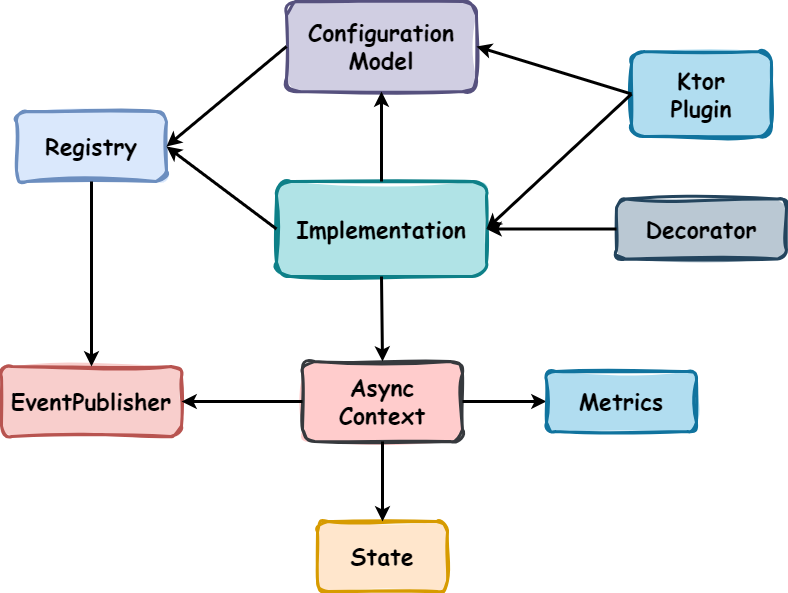
\includegraphics[width=0.8\textwidth]{../figures/03_mechanism-model}
    \caption{Mechanism Model}
    \label{fig:mechanism-model}
\end{figure}

\subsection{Configuration Design}\label{subsec:configuration-design}

Since the start of the project, the Configuration component was designed to use the builder pattern~\cite{wiki:builder-pattern}.
This way, separating the configuration definition (mutable) from the configuration usage (immutable).
However, the initial implementation had a limitation: it was not possible to override a configuration object (i.e., create a new configuration object based on an existing one and only change a few properties while keeping the rest).

In order to overcome this limitation, the Configuration component, and more specifically, its builder, was redesigned
to always receive a base configuration object in its creation.
This modification allows for incremental configuration, essentially following the pattern: \texttt{config(default/initial) -> configBuilder -> config -> configBuilder -> config -> (...)}~\ref{ch:appendix-config-builder}.

\subsection{Mechanism Execution Context}\label{subsec:mechanism-execution-context}

The mechanism's execution context is crucial for ensuring proper operation across synchronous and asynchronous environments.
Since the mechanisms are designed to be cross-platform, the execution context must be flexible and support asynchronous operations, particularly for JavaScript, one of the supported targets (see Section~\ref{sec:supported-targets}), which is single-threaded and requires asynchronous (non-blocking) operations.

Independent of the execution environment, the execution context is one of the following forms:

\begin{itemize}
    \item \textbf{Per Mechanism}: A new execution context is created when the mechanism itself is instantiated (e.g., the Circuit Breaker mechanism has a single execution context for managing the circuit state, as multiple callers can interact with the mechanism at the same time).
    \item \textbf{Per Decoration}: When a decorator is applied to an operation, it creates a new execution context specific to that decoration, before invoking the underlying operation.
    \item \textbf{Per Method Invocation}: A new execution context is created each time the decorated method is invoked.
    This is the most granular form of execution context, providing isolation for each method call.
    If the underlying operation is thread-safe, then this form of execution context is also thread-safe, as only the calling thread executes the context (e.g., the Retry mechanism creates a new execution context for each underlying operation invocation).
\end{itemize}


\section{Ktor Integration}\label{sec:ktor-integration}

Integration with Ktor was considered from the beginning of the project, because Ktor:
\begin{itemize}
    \item provides a flexible pipeline-based architecture, which allows for integration of custom behavior;
    \item is an official JetBrains product;
    \item is also a multiplatform framework, although server-side is limited to the JVM and Native targets~\cite{ktor-server-platforms}.
\end{itemize}

Additionally, integrating with another library or framework (beyond just Ktor) provided a real-world use case for the implemented mechanisms and presented a development exercise.
The challenge was not only integrate the library with a third-party framework, but also ensure that the implemented mechanisms are well-equipped to handle different scenarios and environments without being dependent on a specific context (e.g., HTTP); and also provide extension points for additional features and customizations that only make sense in a specific context (e.g., retrying on server responses with specific status codes).

\subsection{Plugin}\label{subsec:plugin}

In Ktor, a plugin is a reusable component that can be installed in an application to extend its functionality.
They represent a way to encapsulate common functionality (e.g., logging, authentication, serialization, etc.) and make it reusable across different applications.
Plugins are installed in the application's pipeline, where they can intercept and modify the request and response processing flow, as the Figure~\ref{fig:ktor-server-architecture} demonstrates for the server side.

\begin{figure}[!htb]
    \centering
    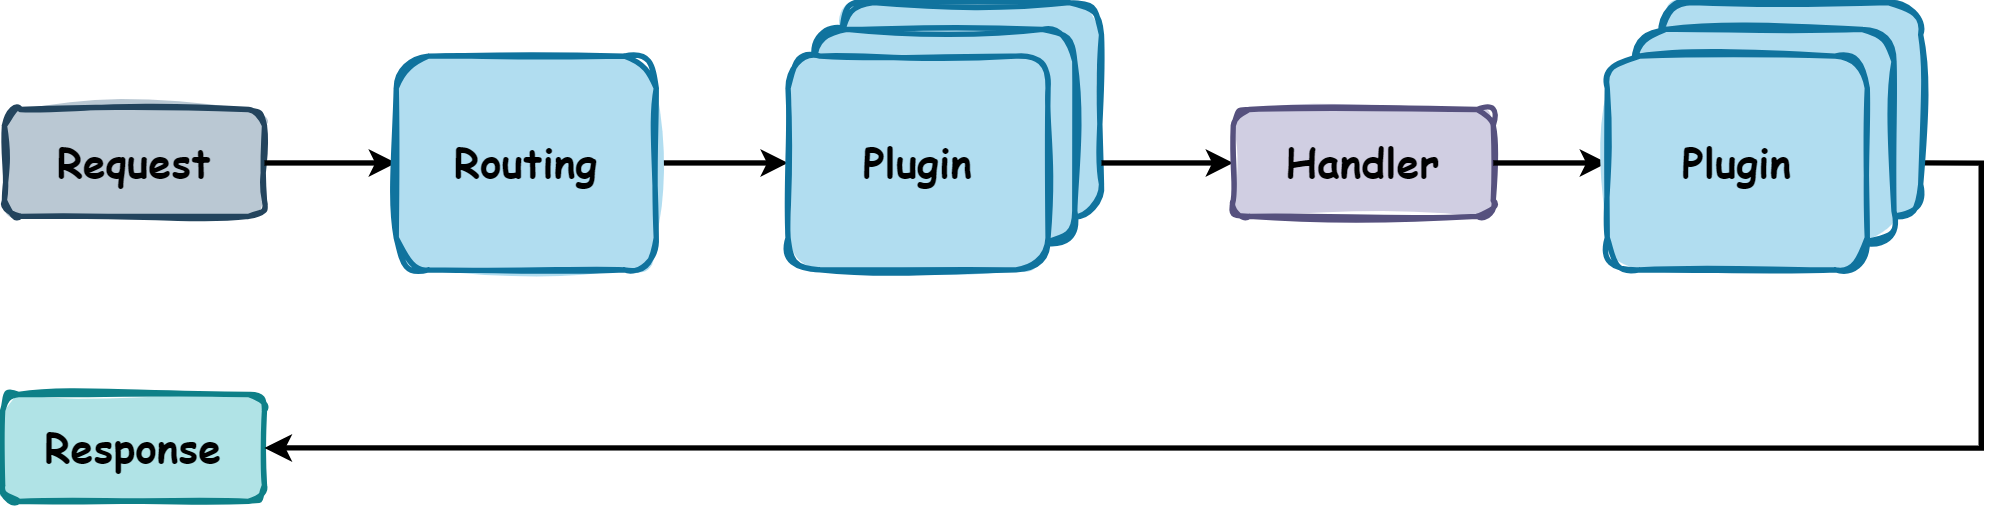
\includegraphics[width=0.8\textwidth]{../figures/03_ktor-server-architecture}
    \caption{Ktor Server Architecture}
    \label{fig:ktor-server-architecture}
\end{figure}

In the server side, as a request comes in, it goes through a series of steps~\cite{ktor-server-plugins}:

\begin{boldenumerate}[topsep=0pt,itemsep=0pt,partopsep=0pt, parsep=0pt]
    \item It is routed to the correct handler via the routing mechanism (which is also a plugin);
    \item Before being handed off to the handler, it goes through one or more Plugins;
    \item The handler (application logic) handles the request;
    \item Before the response is sent to the client, it goes through one or more Plugins
\end{boldenumerate}

\subsection{Pipeline}\label{subsec:pipeline}

A Pipeline, represented in Figure~\ref{fig:ktor-pipeline}, is a collection of zero or more interceptors, grouped in one or more ordered phases.
Each interceptor can perform custom logic before and after processing a request.

\begin{figure}[!htb]
    \centering
    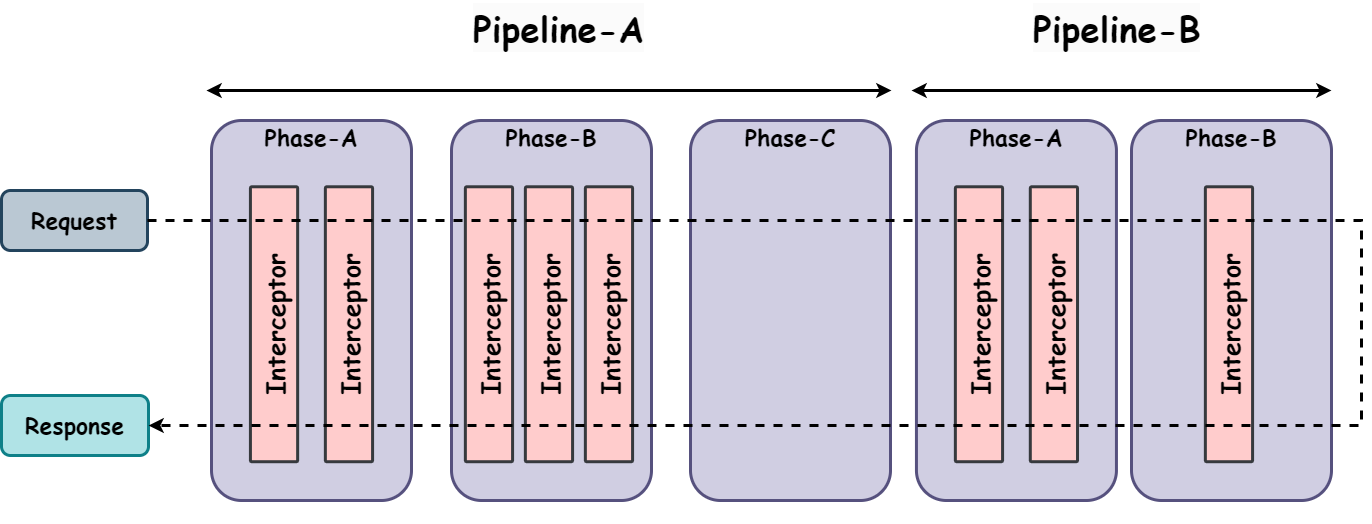
\includegraphics[width=0.8\textwidth]{../figures/03_ktor-pipeline}
    \caption{Ktor Pipeline Example}
    \label{fig:ktor-pipeline}
\end{figure}

A plugin is also an interceptor, but an interceptor is not a plugin.
While an interceptor is a function block that can be added to intercept a specific pipeline phase and perform custom logic; a plugin is a collection of zero or more interceptors mixed with external configuration and other logic (e.g., add more pipeline phases) in a single reusable component.

Both client and server sides have pipelines, but they differ in terms of their phases and purposes.
Tables~\ref{tab:ktor-server-pipelines} and~\ref{tab:ktor-client-pipelines} show the phases of the server and client pipelines, respectively.

\begin{table}[!htb]
    \centering
    \caption{Ktor Server Pipelines}
    \label{tab:ktor-server-pipelines}
    \vspace{0.3cm}
    \begin{tabular}{|l|p{6cm}|p{5cm}|p{5cm}|}
        \hline
        \textbf{Pipeline}  & \textbf{Description}                        & \textbf{Phases}                                                               \\ \hline
        ApplicationSend    & Responsible for sending responses           & Before, Transform, Render, Content-Encoding, Transfer-Encoding, After, Engine \\ \hline
        ApplicationReceive & Responsible for receiving requests          & Before, Transform, After                                                      \\ \hline
        ApplicationCall    & Responsible for executing application calls & Setup, Monitoring, Plugins, Call, Fallback                                    \\ \hline
    \end{tabular}
\end{table}

\begin{table}[!htb]
    \centering
    \caption{Ktor Client Pipelines}
    \label{tab:ktor-client-pipelines}
    \vspace{0.3cm}
    \begin{tabular}{|l|p{6cm}|p{5cm}|p{5cm}|}
        \hline
        \textbf{Pipeline} & \textbf{Description}                             & \textbf{Phases}                            \\ \hline
        HttpRequest       & Processes all requests sent by the client        & Before, State, Transform, Render, Send     \\ \hline
        HttpSend          & Used for send a request                          & Before, State, Monitoring, Engine, Receive \\ \hline
        HttpReceive       & Used for receiving a response without processing & Before, State, After                       \\ \hline
        HttpResponse      & Used for processing responses                    & Receive, Parse, Transform, State, After    \\ \hline
    \end{tabular}
\end{table}

\subsection{Custom Plugins}\label{subsec:custom-plugins}

Ktor provides a custom plugin API that allows developers to create their own plugins in both client and server sides.

Since Ktor \texttt{2.0.0}, the custom plugin API has been simplified~\cite{ktor-server-custom-plugins, ktor-client-custom-plugins} and no longer requires an understanding of internal Ktor concepts, such as pipelines, phases, etc.
Instead, developers have access to different stages of handling requests and responses using general handlers (e.g., \texttt{onCallReceive}, and \texttt{onCallRespond}), which intercept the related phases of the pipeline.

\section{Development Roadmap}\label{sec:development-roadmap}

Originally, the project was planned to be developed in a horizontal manner, where all mechanisms would be implemented for all targets at the same time, tested, and then integrated with Ktor.

However, due to the complexity of the mechanisms and the need to ensure that they are correctly implemented and tested
in other contexts, the development strategy was changed to a vertical approach.

For each mechanism, the following steps are taken:
\begin{boldenumerate}[topsep=0pt,itemsep=0pt,partopsep=0pt, parsep=0pt]
    \item \textbf{Mechanism Model Implementation}: Implement the Mechanism Model for a specific mechanism, including all of its components.
    \item \textbf{Tests}: Write tests for the implemented Mechanism Model components.
    \item \textbf{All Targets Support}: Ensure that the implemented Mechanism Model components work correctly for all targets.
    \item \textbf{Ktor Plugin}: Implement the Ktor Plugin for the mechanism.
    \item \textbf{Ktor Plugin Tests}: Write tests for the implemented Ktor Plugin.
    Due to time constraints, unit tests were not conducted; however, integration tests~\cite{software-test-types} were performed using a real Ktor application.
\end{boldenumerate}
